\documentclass[journal]{vgtc} 
\usepackage{hs-vis_ss10}


%% Please note that the use of figures other than the optional teaser
%% is not permitted on the first page of the journal version.  Figures
%% should begin on the second page and be in CMYK or Grey scale
%% format, otherwise, colour shifting may occur during the printing
%% process.  Papers submitted with figures other than the optional
%% teaser on the first page will be refused.

%% These three lines bring in essential packages: ``mathptmx'' for
%% Type 1 typefaces, ``graphicx'' for inclusion of EPS figures. and
%% ``times'' for proper handling of the times font family.

\usepackage{mathptmx} 
\usepackage{graphicx}
\usepackage{times}

%% allow for this line if you want the electronic option to work
%% properly
\vgtcinsertpkg


%% author name
\author{Moritz Hamann}

%% paper title
\title{Clustering of dynamic graphs}

%% short title for header
\shorttitle{Clustering of dynamic graphs}


%% Abstract section.
\abstract{%
This paper presents a summary about various techniques to detect and identify densely connected
nodes in a graph, so called clusters. In the first part, we introduce the concept of clusters for
static graphs alongside their main properties. For dynamic graphs with time varying edge connections,
these cluster may be subject to change with every time step. Therefore additional characteristics
have to be introduced.

The second part describes two methods to detect, identify and track cluster in a dynamic graph.
A common solution for this problem is the clustering of a static graph at each time step, and the
identification of the same clusters over multiple time steps. A method is presented to track these
clusters, which is independent of the underlying static graph clustering algorithm.
Furthermore, we describe an extension of the k-clique percolation algorithm to dynamic graphs.

Finally, the clique percolation algorithm is applied to two different real world networks, which
yields interesting result about group dynamics, with regards to the correlation of various group
properties.
} % end of abstract


%% Uncomment below to include a (optional) teaser figure.
\teaser{ \centering
  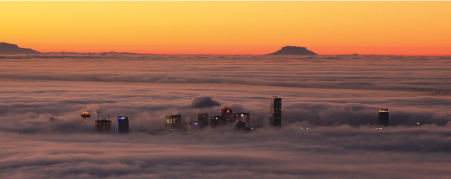
\includegraphics[width=16cm]{images/CypressView}
  \caption{In den Wolken: Vancouver von Cypress Mountain. Auf der
    ersten Seite d"urfen keine Grafiken au"ser dieser optionalen
    Aufmachgrafik (Teaser) abgebildet sein.}
}


%%%%%%%%%%%%%%%%%%%%%%%%%%%%%%%%%%%%%%%%%%%%%%%%%%%%%%%%%%%%%%%%
%%%%%%%%%%%%%%%%%%%%%% START OF THE PAPER %%%%%%%%%%%%%%%%%%%%%%
%%%%%%%%%%%%%%%%%%%%%%%%%%%%%%%%%%%%%%%%%%%%%%%%%%%%%%%%%%%%%%%%%

\begin{document}

%% The ``\maketitle'' command must be the first command after the
%% ``\begin{document}'' command. It prepares and prints the title
%%   block.

%%   the only exception to this rule is the \firstsection command
\firstsection{Motivation}
\maketitle

  Das mathematische Konzept der Graphen ist ein essentielles 
  Modellierungswerkzeug in der Informatik. Nicht nur lassen sich damit
  verschiedenste Datenstrukturen anschaulich dargestellen, sondern
  mit ihrer Hilfe lassen sich auch jegliche Beziehungen zwischen einzelnen
  Objekten oder Prozessen in einem Netzwerk modellieren und untersuchen.
  Aus diesem Grund sind sie heutzutage nicht nur in der klassischen Informatik
  sowie in der Mathematik zu finden, sondern haben auch in vielen anderen
  Wissenschaften ihren Einzug erhalten. So werden sie genutzt um die
  Gruppendynamik in biologischen Netzwerken zu beschreiben, dienen
  als Kontrollalgorithmen für Multiagenten Systeme [?] und beschreiben
  Kommunikationsmuster in sozialen Netzwerken.
  
  Um die Eigenschaften sehr großer Netzwerke analytisch untersuchen zu können,
  werden häufig Zufallsgraphen nach dem Model von Edgar Gilbert (nachweise?) oder
  Erdos-Renyi verwendet. Diese Graphen haben die Besonderheit, dass die 
  Wahrscheinlichkeit für eine Verbindung zwischen je zwei Knoten im 
  gesammten Netzwerk konstant ist. Dadurch ensteht ein gleichmäßiger Graph,
  dessen Gradverteilung binomial verteilt sind, und somit die meisten Knoten 
  die gleiche Anzahl an Kanten haben. Mit Hilfe der Wahrscheinlichkeitstheorie,
  lassen sich nun die Eigenschaften dieser Graphen auch für eine sehr hohe Anzahl
  an Knoten bestimmen und untersuchen.
  
  Allerdings haben Untersuchungen von realen Netzen gezeigt (nachweis), dass sich
  diese in den meisten Fällen von Zufallsgraphen unterscheiden. Reale Netzwerke sind
  häufig sogenannte Skalenfreie Netze (im Englischen 'Scale-free networks'), in 
  denen die Anzahl der Verbindungen pro Knoten nicht binomial verteilt ist, sonder nach einem
  Potentzgesetz. Dadurch einsteht ein Netzwerk, in dem einzelne wenige Knoten eine große
  Anzahl an Verknüpfungen aufweisen, doch die Mehrzahl der Knoten weniger stark verknüpft ist. 
  Weiterhin ist die Kantenverteilung zwischen den Knoten auch lokal sehr inhomogen, so dass sich 
  Teilgraphen ausbilden, deren Knoten untereinander sehr stark bis komplett verknüpft sind.
  Diese Teilgraphen werden auch 'Cluster' genannt.
  
  Gerade diese Cluster sind für viele Anwendungsgebiete interessant. 
  Aber auch in sozialen Netzwerken ist die Clusteranalyse essentiel. Betrachtet man die Freundschafts
  Beziehungen in einem solchen Graph, lassen sich aus lokalen Cluster unter anderem
  Rückschlüße auf gemeinsame Interessen, Wohnorte oder Arbeitsplätze ziehen.
  Diese Informationen bieten dem soziale Marketing eine bis vor kurzem unbekannte Menge
  an Möglichkeiten ihre Produkte zielgerichteter und persönlicher zu vermarkten.
  Aber auch in dynamischen Graphen, in denen Knoten und Kanten sehr häufig wechseln können,
  ist es wichtig Cluster zu finden. Betrachtet man den Verbindungsgraph eines dezentralen, 
  kabellosen Ad-Hoc Netzwerks, so lassen sich mit Hilfe von Clustering Verfahren 
  Teilnetze finden die geographisch
  Eine zusätzliche Herrausforderung zur eigentlichen Clusteranalyse ist hierbei allerdings
  
  Diese Arbeit gibt einen Überblick über die Eigenschaften dieser Cluster, ihr

\section{Grundlagen}
  was sind cluster, ueberlabende cluster, definition?
  \subsection{Eigenschaften von Clustern}
  \subsection{Properties of dynamic graphs}
  
\section{Clustering in static graphs}
  \subsection{Clique percolation}
  \subsection{modularity function clustering?}

\section{Clustering in dynamic graphs}
  \subsection{Extension of clique percolation}
  \subsection{Time step Clustering}

\section{maybe visualization of dynamic graphs}
  
\section{Group Evolution (results)}
 
\section{Conclusion}


\subsection{Abbildungen und Tabellen}

Alle Abbildungen (siehe Abb.\ \ref{fig:sample}) und Tabellen (Tabelle\
\ref{tab:vis_accept}) sollten zentriert sein
(\verb|\centering|). Abbildungen "uber beide Textspalten
(Abb. \ref{fig:multicolumn}) k"onnen mit
\verb|\begin{figure*}|\ldots\verb|\end{figure*}| eingef"ugt werden.

\subsection{Referenzen}

Literaturangaben wie beispielsweise Levoy \cite{levoy:1989:DSV} werden
mit Hilfe von BibTeX erzeugt. Dazu werden die Referenzen in die
Literaturliste (hier \emph{literatur.bib}) eingetragen und
entsprechend mit \verb|\cite| referenziert.

\subsection{\LaTeX-"Ubersetzung}

Die \LaTeX-Datei kann mit \emph{latex} oder \emph{pdflatex} "ubersetzt
werden. Dabei ist zu beachten, dass f"ur die "Ubersetzung mit
\emph{latex} die Grafiken in Postscript (eps) vorliegen, f"ur
\emph{pdflatex} entsprechend als jpg, png oder pdf.  Der Ablauf ist
dabei der folgende:
\begin{enumerate}
\item \verb|pdflatex <quelldatei.tex>|
\item \verb|bibtex <quelldatei>|
\item \verb|pdflatex <quelldatei.tex>| (evtl. mehrfach)
\end{enumerate}
Alternativ kann auch das mitgelieferte Makefile verwendet werden.





Lorem ipsum dolor sit amet, consetetur sadipscing elitr, sed diam
nonumy eirmod tempor invidunt ut labore et dolore magna aliquyam erat,
sed diam voluptua. At vero eos et accusam et justo duo dolores et ea
rebum. Stet clita kasd gubergren, no sea takimata sanctus est Lorem
ipsum dolor sit amet. Lorem ipsum dolor sit amet, consetetur
sadipscing elitr, sed diam nonumy eirmod tempor invidunt ut labore et
dolore magna aliquyam erat, sed diam
voluptua~\cite{kitware2003,Max:1995:OMF}. At vero eos et accusam et
justo duo dolores et ea rebum. Stet clita kasd gubergren, no sea
takimata sanctus est Lorem ipsum dolor sit amet. Lorem ipsum dolor sit
amet, consetetur sadipscing elitr, sed diam nonumy eirmod tempor
invidunt ut labore et dolore magna aliquyam erat, sed diam
voluptua. At vero eos et accusam et justo duo dolores et ea
rebum. Stet clita kasd gubergren, no sea takimata sanctus est Lorem
ipsum dolor sit amet.

Duis autem vel eum iriure dolor in hendrerit in vulputate velit esse
molestie consequat, vel illum dolore eu feugiat nulla facilisis at
vero eros et accumsan et iusto odio dignissim qui blandit praesent
luptatum zzril delenit augue duis dolore te feugait nulla
facilisi~\cite{notes2002}. Lorem ipsum dolor sit amet, consectetuer
adipiscing elit, sed diam nonummy nibh euismod tincidunt ut laoreet
dolore magna aliquam erat volutpat.

Ut wisi enim ad minim veniam, quis nostrud exerci tation ullamcorper
suscipit lobortis nisl ut aliquip ex ea commodo consequat. Duis autem
vel eum iriure dolor in hendrerit in vulputate velit esse molestie
consequat, vel illum dolore eu feugiat nulla facilisis at vero eros et
accumsan et iusto odio dignissim qui blandit praesent luptatum zzril
delenit augue duis dolore te feugait nulla facilisi.



Lorem ipsum dolor sit amet, consetetur sadipscing elitr, sed diam
nonumy eirmod tempor invidunt ut labore et dolore magna aliquyam erat,
sed diam voluptua. At vero eos et accusam et justo duo dolores et ea
rebum. Stet clita kasd gubergren, no sea takimata sanctus est Lorem
ipsum dolor sit amet. Lorem ipsum dolor sit amet, consetetur
sadipscing elitr, sed diam nonumy eirmod tempor invidunt ut labore et
dolore magna aliquyam erat, sed diam voluptua. At vero eos et accusam
et justo duo dolores et ea rebum. Stet clita kasd gubergren, no sea
takimata sanctus est Lorem ipsum dolor sit amet. Lorem ipsum dolor sit
amet, consetetur sadipscing elitr, sed diam nonumy eirmod tempor
invidunt ut labore et dolore magna aliquyam erat, sed diam
voluptua. At vero eos et accusam et justo duo dolores et ea
rebum~\cite{ware:2004:IVP}. Stet clita kasd gubergren, no sea takimata
sanctus est Lorem ipsum dolor sit amet.

Duis autem vel eum iriure dolor in hendrerit in vulputate velit esse
molestie consequat, vel illum dolore eu feugiat nulla facilisis at
vero eros et accumsan et iusto odio dignissim qui blandit praesent
luptatum zzril delenit augue duis dolore te feugait nulla
facilisi. Lorem ipsum dolor sit amet, consectetuer adipiscing elit,
sed diam nonummy nibh euismod tincidunt ut laoreet dolore magna
aliquam erat volutpat~\cite{kindlmann:1999:SAG}.

Ut wisi enim ad minim veniam, quis nostrud exerci tation ullamcorper
suscipit lobortis nisl ut aliquip ex ea commodo
consequat~\cite{levoy:1989:DSV}. Duis autem vel eum iriure dolor in
hendrerit in vulputate velit esse molestie consequat, vel illum dolore
eu feugiat nulla facilisis at vero eros et accumsan et iusto odio
dignissim qui blandit praesent luptatum zzril delenit augue duis
dolore te feugait nulla facilisi.

Lorem ipsum dolor sit amet, consetetur sadipscing elitr, sed diam
nonumy eirmod tempor invidunt ut labore et dolore magna aliquyam erat,
sed diam voluptua. At vero eos et accusam et justo duo dolores et ea
rebum. Stet clita kasd gubergren, no sea takimata sanctus est Lorem
ipsum dolor sit amet. Lorem ipsum dolor sit amet, consetetur
sadipscing elitr, sed diam nonumy eirmod tempor invidunt ut labore et
dolore magna aliquyam erat, sed diam voluptua. At vero eos et accusam
et justo duo dolores et ea rebum. Stet clita kasd gubergren, no sea
takimata sanctus est Lorem ipsum dolor sit amet. Lorem ipsum dolor sit
amet, consetetur sadipscing elitr, sed diam nonumy eirmod tempor
invidunt ut labore et dolore magna aliquyam erat, sed diam
voluptua. At vero eos et accusam et justo duo dolores et ea
rebum. Stet clita kasd gubergren, no sea takimata sanctus est Lorem
ipsum dolor sit amet.

Lorem ipsum dolor sit amet, consetetur sadipscing elitr, sed diam
nonumy eirmod tempor invidunt ut labore et dolore magna aliquyam erat,
sed diam voluptua. At vero eos et accusam et justo duo dolores et ea
rebum. Stet clita kasd gubergren, no sea takimata sanctus est Lorem
ipsum dolor sit amet. Lorem ipsum dolor sit amet, consetetur
sadipscing elitr, sed diam nonumy eirmod tempor invidunt ut labore et
dolore magna aliquyam erat, sed diam voluptua. At vero eos et accusam
et justo duo dolores et ea rebum. Stet clita kasd gubergren, no sea
takimata sanctus est Lorem ipsum dolor sit amet. Lorem ipsum dolor sit
amet, consetetur sadipscing elitr, sed diam nonumy eirmod tempor
invidunt ut labore et dolore magna aliquyam erat, sed diam
voluptua. At vero eos et accusam et justo duo dolores et ea
rebum. Stet clita kasd gubergren, no sea takimata sanctus est Lorem
ipsum dolor sit amet.

Lorem ipsum dolor sit amet, consetetur sadipscing elitr, sed diam
nonumy eirmod tempor invidunt ut labore et dolore magna aliquyam erat,
sed diam voluptua. At vero eos et accusam et justo duo dolores et ea
rebum. Stet clita kasd gubergren, no sea takimata sanctus est Lorem
ipsum dolor sit amet. Lorem ipsum dolor sit amet, consetetur
sadipscing elitr, sed diam nonumy eirmod tempor invidunt ut labore et
dolore magna aliquyam erat, sed diam voluptua.


\begin{figure}[tb]
  \centering
  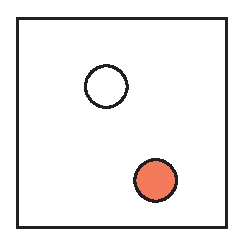
\includegraphics[width=1.5in]{sample}
  \caption{\label{fig:sample} Beispielillustration.}
\end{figure}

\begin{equation}
  \sum_{j=1}^{z} j = \frac{z(z+1)}{2}
\end{equation}

Lorem ipsum dolor sit amet, consetetur sadipscing elitr, sed diam
nonumy eirmod tempor invidunt ut labore et dolore magna aliquyam erat,
sed diam voluptua. At vero eos et accusam et justo duo dolores et ea
rebum. Stet clita kasd gubergren, no sea takimata sanctus est Lorem
ipsum dolor sit amet. Lorem ipsum dolor sit amet, consetetur
sadipscing elitr, sed diam nonumy eirmod tempor invidunt ut labore et
dolore magna aliquyam erat, sed diam voluptua. At vero eos et accusam
et justo duo dolores et ea rebum. Stet clita kasd gubergren, no sea
takimata sanctus est Lorem ipsum dolor sit amet. Lorem ipsum dolor sit
amet, consetetur sadipscing elitr, sed diam nonumy eirmod tempor
invidunt ut labore et dolore magna aliquyam erat, sed diam
voluptua. At vero eos et accusam et justo duo dolores et ea
rebum. Stet clita kasd gubergren, no sea takimata sanctus est Lorem
ipsum dolor sit amet.

Lorem ipsum dolor sit amet, consetetur sadipscing elitr, sed diam
nonumy eirmod tempor invidunt ut labore et dolore magna aliquyam erat,
sed diam voluptua. At vero eos et accusam et justo duo dolores et ea
rebum. Stet clita kasd gubergren, no sea takimata sanctus est Lorem
ipsum dolor sit amet. Lorem ipsum dolor sit amet, consetetur
sadipscing elitr, sed diam nonumy eirmod tempor invidunt ut labore et
dolore magna aliquyam erat, sed diam voluptua. At vero eos et accusam
et justo duo dolores et ea rebum. Stet clita kasd gubergren, no sea
takimata sanctus est Lorem ipsum dolor sit amet. Lorem ipsum dolor sit
amet, consetetur sadipscing elitr, sed diam nonumy eirmod tempor
invidunt ut labore et dolore magna aliquyam erat, sed diam
voluptua. At vero eos et accusam et justo duo dolores et ea
rebum. Stet clita kasd gubergren, no sea takimata sanctus est Lorem
ipsum dolor sit amet.

\begin{table}
  %% Table captions on top in journal version
  \caption{\label{tab:vis_accept} Vis Paper Acceptance Rate}
  \scriptsize
  \begin{center}
    \begin{tabular}{cccc}
      Year & Submitted & Accepted & Accepted (\%)\\
      \hline
      1994 &  91 & 41 & 45.1\\
      1995 & 102 & 41 & 40.2\\
      1996 & 101 & 43 & 42.6\\
      1997 & 117 & 44 & 37.6\\
      1998 & 118 & 50 & 42.4\\
      1999 & 129 & 47 & 36.4\\
      2000 & 151 & 52 & 34.4\\
      2001 & 152 & 51 & 33.6\\
      2002 & 172 & 58 & 33.7\\
      2003 & 192 & 63 & 32.8\\
      2004 & 167 & 46 & 27.6\\
      2005 & 268 & 88 & 32.8\\
      2006 & 228 & 63 & 27.6
    \end{tabular}
  \end{center}
\end{table}


Lorem ipsum dolor sit amet, consetetur sadipscing elitr, sed diam
nonumy eirmod tempor invidunt ut labore et dolore magna aliquyam erat,
sed diam voluptua. At vero eos et accusam et justo duo dolores et ea
rebum. Stet clita kasd gubergren, no sea takimata sanctus est Lorem
ipsum dolor sit amet. Lorem ipsum dolor sit amet, consetetur
sadipscing elitr, sed diam nonumy eirmod tempor invidunt ut labore et
dolore magna aliquyam erat, sed diam voluptua. At vero eos et accusam
et justo duo dolores et ea rebum. Stet clita kasd gubergren, no sea
takimata sanctus est Lorem ipsum dolor sit amet.

\begin{figure*}[tb]
  \centering
  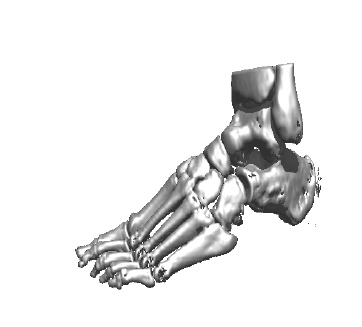
\includegraphics[width=4cm]{images/foot1}\hfill
  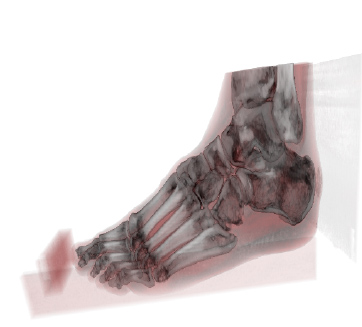
\includegraphics[width=4cm]{images/foot2}\hfill
  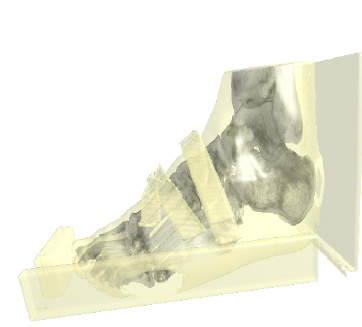
\includegraphics[width=4cm]{images/foot3}\hfill
  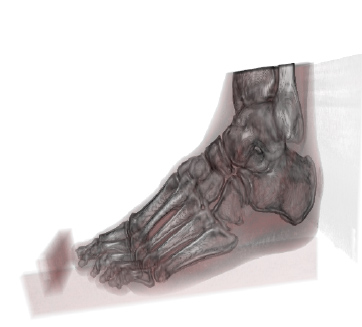
\includegraphics[width=4cm]{images/foot4}
  \caption{Illustration "uber beide Textspalten hinweg. Auch
    Illustrationen m"ussen entsprechend den Quellen gekennzeichnet
    werden. \cite{strengert2006spectral}}
  \label{fig:multicolumn}
\end{figure*}


Lorem ipsum dolor sit amet, consetetur sadipscing elitr, sed diam
nonumy eirmod tempor invidunt ut labore et dolore magna aliquyam erat,
sed diam voluptua. At vero eos et accusam et justo duo dolores et ea
rebum. Stet clita kasd gubergren, no sea takimata sanctus est Lorem
ipsum dolor sit amet. Lorem ipsum dolor sit amet, consetetur
sadipscing elitr, sed diam nonumy eirmod tempor invidunt ut labore et
dolore magna aliquyam erat, sed diam voluptua. At vero eos et accusam
et justo duo dolores et ea rebum. Stet clita kasd gubergren, no sea
takimata sanctus est Lorem ipsum dolor sit amet. Lorem ipsum dolor sit
amet, consetetur sadipscing elitr, sed diam nonumy eirmod tempor
invidunt ut labore et dolore magna aliquyam erat, sed diam
voluptua. At vero eos et accusam et justo duo dolores et ea
rebum. Stet clita kasd gubergren, no sea takimata sanctus est Lorem
ipsum dolor sit amet.


\subsection{Mezcal Head}

Duis autem~\cite{Lorensen:1987:MCA} vel eum iriure dolor in hendrerit
in vulputate velit esse molestie consequat, vel illum dolore eu
feugiat nulla facilisis at vero eros et accumsan et iusto odio
dignissim qui blandit praesent luptatum zzril delenit augue duis
dolore te feugait nulla facilisi. Lorem ipsum dolor sit amet,
consectetuer adipiscing elit, sed diam nonummy nibh euismod tincidunt
ut laoreet dolore magna aliquam erat volutpat%
\footnote{Fu"snoten erscheinen an der Unterkante der Spalte. Sie
  sollten jedoch vermieden werden, da der Lesefluss gest"ort wird.}.


\subsubsection{Ejector Seat Reservation}

Ut wisi enim ad minim veniam, quis nostrud exerci tation ullamcorper
suscipit lobortis nisl ut aliquip ex ea commodo
consequat~\cite{Nielson:1991:TAD}. Duis autem vel eum iriure dolor in
hendrerit in vulputate velit esse molestie consequat, vel illum dolore
eu feugiat nulla facilisis at vero eros et accumsan et iusto odio
dignissim qui blandit praesent luptatum zzril delenit augue duis
dolore te feugait nulla facilisi.

\paragraph{Rejected Ejector Seat Reservation}

Ut wisi enim ad minim veniam, quis nostrud exerci tation ullamcorper
suscipit lobortis nisl ut aliquip ex ea commodo consequat. Duis autem
vel eum iriure dolor in hendrerit in vulputate velit esse molestie

\section{Conclusion}

Lorem ipsum dolor sit amet, consetetur sadipscing elitr, sed diam
nonumy eirmod tempor invidunt ut labore et dolore magna aliquyam erat,
sed diam voluptua. At vero eos et accusam et justo duo dolores et ea
rebum. Stet clita kasd gubergren, no sea takimata sanctus est Lorem
ipsum dolor sit amet. Lorem ipsum dolor sit amet, consetetur
sadipscing elitr, sed diam nonumy eirmod tempor invidunt ut labore et
dolore magna aliquyam erat, sed diam voluptua. At vero eos et accusam
et justo duo dolores et ea rebum. Stet clita kasd gubergren, no sea
takimata sanctus est Lorem ipsum dolor sit amet. Lorem ipsum dolor sit
amet, consetetur sadipscing elitr, sed diam nonumy eirmod tempor
invidunt ut labore et dolore magna aliquyam erat, sed diam
voluptua. At vero eos et accusam et justo duo dolores et ea
rebum. Stet clita kasd gubergren, no sea takimata sanctus est Lorem
ipsum dolor sit amet.

Lorem ipsum dolor sit amet, consetetur sadipscing elitr, sed diam
nonumy eirmod tempor invidunt ut labore et dolore magna aliquyam erat,
sed diam voluptua. At vero eos et accusam et justo duo dolores et ea
rebum. Stet clita kasd gubergren, no sea takimata sanctus est Lorem
ipsum dolor sit amet. Lorem ipsum dolor sit amet, consetetur
sadipscing elitr, sed diam nonumy eirmod tempor invidunt ut labore et
dolore magna aliquyam erat, sed diam voluptua. At vero eos et accusam
et justo duo dolores et ea rebum.


\bibliographystyle{abbrv}
%% use following if all content of bibtex file should be shown
% \nocite{*}
\bibliography{literatur}
\end{document}
